""
\documentclass[a4paper,12pt]{article}
\usepackage[utf8]{inputenc}
\usepackage[spanish]{babel}
\usepackage{graphicx}
\usepackage{geometry}
\geometry{margin=2.5cm}
\title{Ejercicios de Codificación Digital con Soluciones}
\author{}
\date{}
\begin{document}
\maketitle


\section*{Ejercicio 1}
Dada la siguiente secuencia binaria: [1, 0, 1, 1, 0], represéntala utilizando la codificación NRZ.



\textbf{SOL:} En NRZ, el '1' se representa con un nivel alto constante y el '0' con un nivel bajo constante. La señal sería: Alto, Bajo, Alto, Alto, Bajo.

\begin{figure}[h!]
\centering
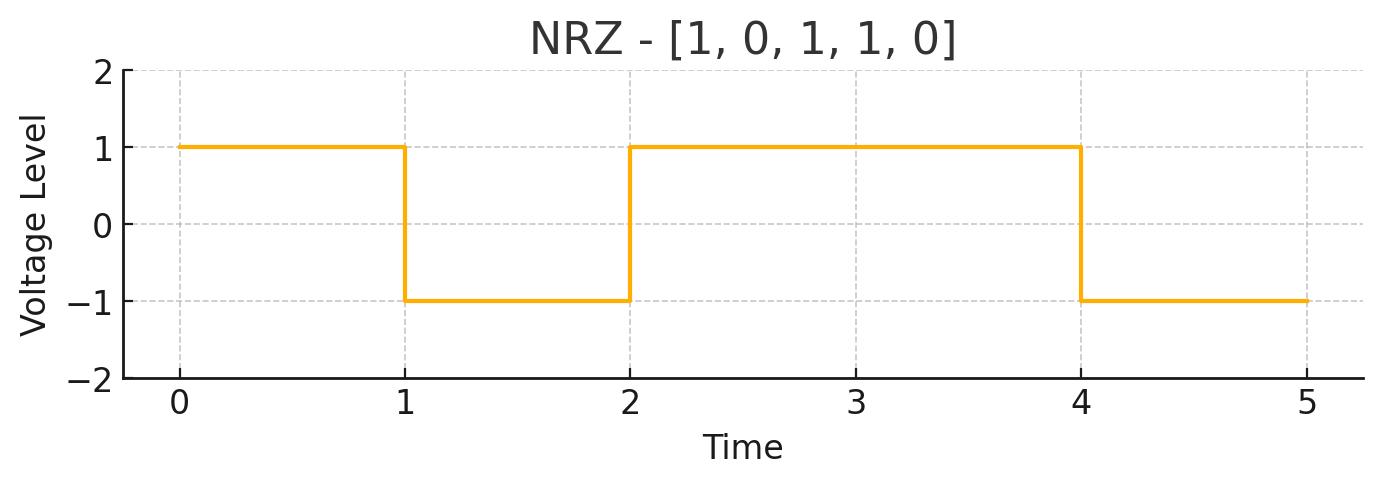
\includegraphics[width=0.85\textwidth]{img/ejercicio_1.png}
\caption{Ejercicio 1: Señal codificada}
\end{figure}
\clearpage


\section*{Ejercicio 2}
Dada la secuencia [0, 1, 0, 0, 1, 1], dibuja la señal correspondiente con codificación Manchester.



\textbf{SOL:} En Manchester: un '0' es Alto→Bajo y un '1' es Bajo→Alto en cada bit. Así que la señal alterna en cada bit con una transición en el centro.

\begin{figure}[h!]
\centering
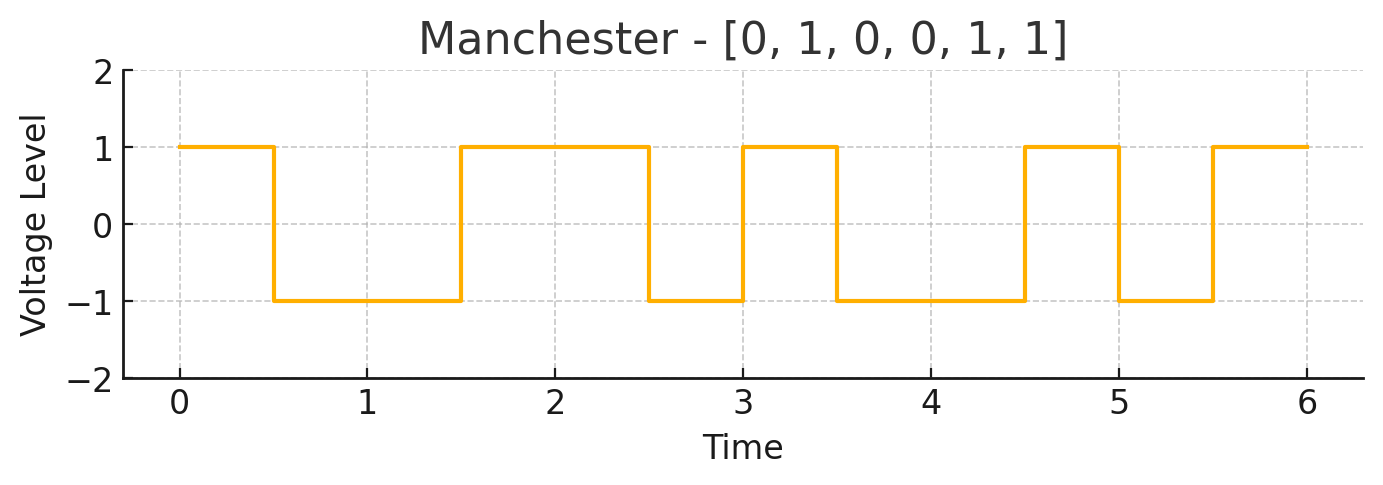
\includegraphics[width=0.85\textwidth]{img/ejercicio_2.png}
\caption{Ejercicio 2: Señal codificada}
\end{figure}
\clearpage



\section*{Ejercicio 4}
Dibuja la señal que resulta de codificar la secuencia [1, 0, 0, 1] utilizando codificación RZ.



\textbf{SOL:} En RZ, cada bit tiene un pulso en la primera mitad y retorno a cero en la segunda mitad. '1' es pulso positivo, ’0’ se representa mediante un pulso negativo o nivel bajo, dependiendo de la convención usada. Se alterna señal y cero cada medio bit.

\begin{figure}[h!]
\centering
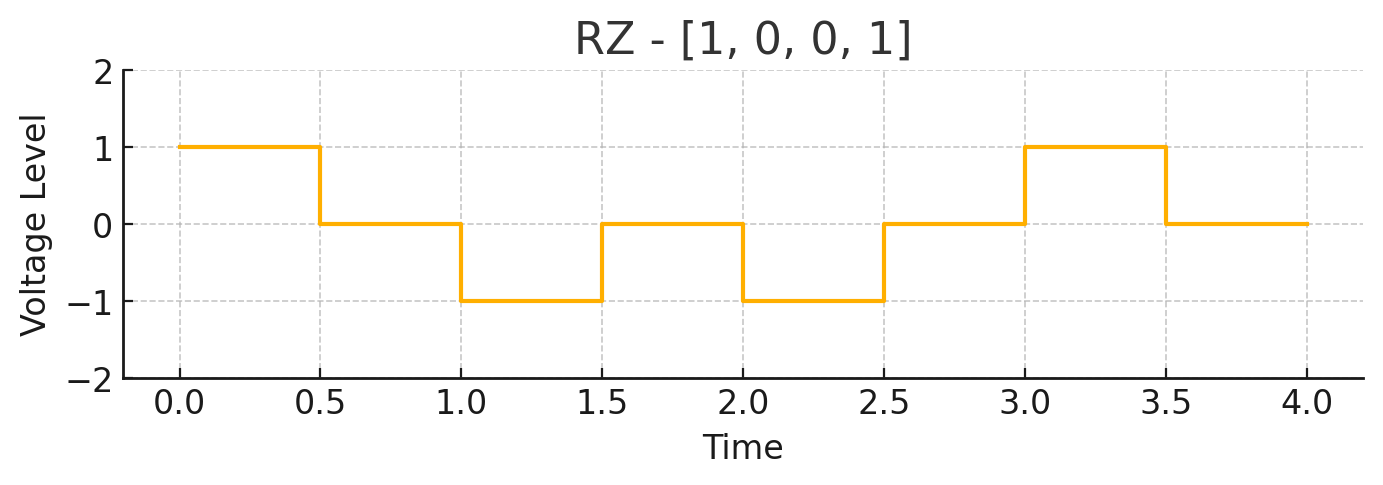
\includegraphics[width=0.85\textwidth]{img/ejercicio_4.png}
\caption{Ejercicio 4: Señal codificada}
\end{figure}
\clearpage


\section*{Ejercicio 5}
¿Cuál es la principal ventaja de la codificación Manchester frente a NRZ?



\textbf{SOL:} La Manchester facilita la sincronización ya que siempre hay una transición en cada bit, mientras que NRZ puede tener largas secuencias sin cambios.




\section*{Ejercicio 7}
Dibuja la señal de la secuencia [0, 1, 1, 0, 1] usando Manchester Diferencial.



\textbf{SOL:} En Manchester Diferencial hay una transición en medio del bit siempre, y el '0' implica transición al inicio. El patrón se calcula según el bit anterior.

\begin{figure}[h!]
\centering
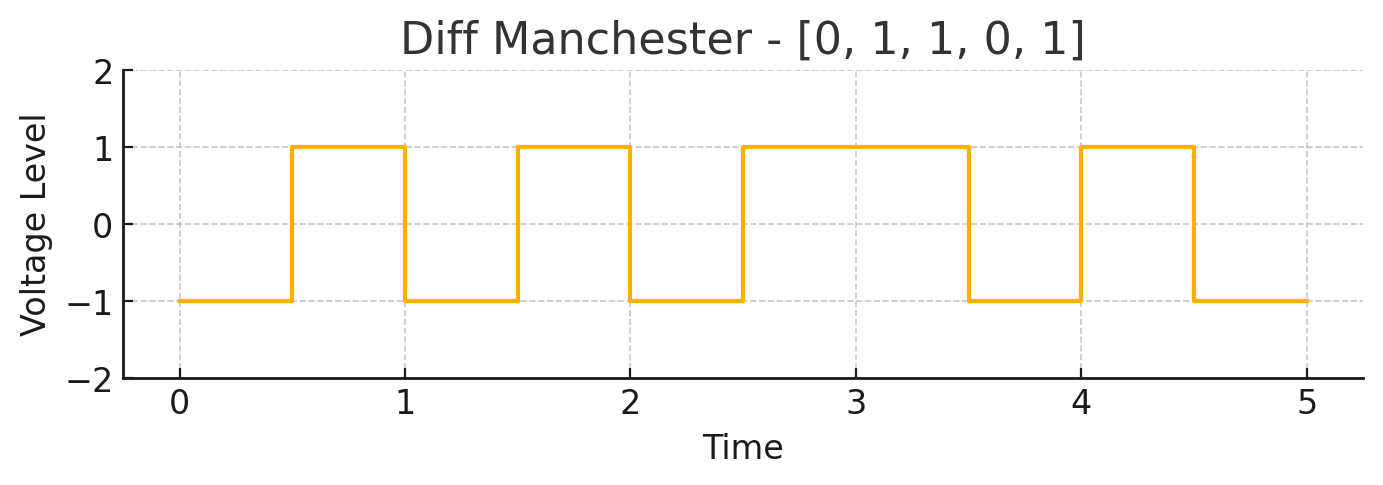
\includegraphics[width=0.85\textwidth]{img/ejercicio_7.png}
\caption{Ejercicio 7: Señal codificada}
\end{figure}
\clearpage


\section*{Ejercicio 8}
En una señal codificada, observas una alternancia clara entre voltajes positivos y negativos para los '1', y niveles planos para los '0'. ¿Qué tipo de codificación es más probable?



\textbf{SOL:} Codificación Bipolar (AMI).



\section*{Ejercicio 9}
Dibuja la señal correspondiente a la secuencia binaria [1, 0, 1, 0, 0, 1, 1] utilizando codificación NRZI.



\textbf{SOL:} En NRZI, se produce una transición al comienzo del bit si es un '1' y no se cambia el nivel si es un '0'.

\begin{figure}[h!]
\centering
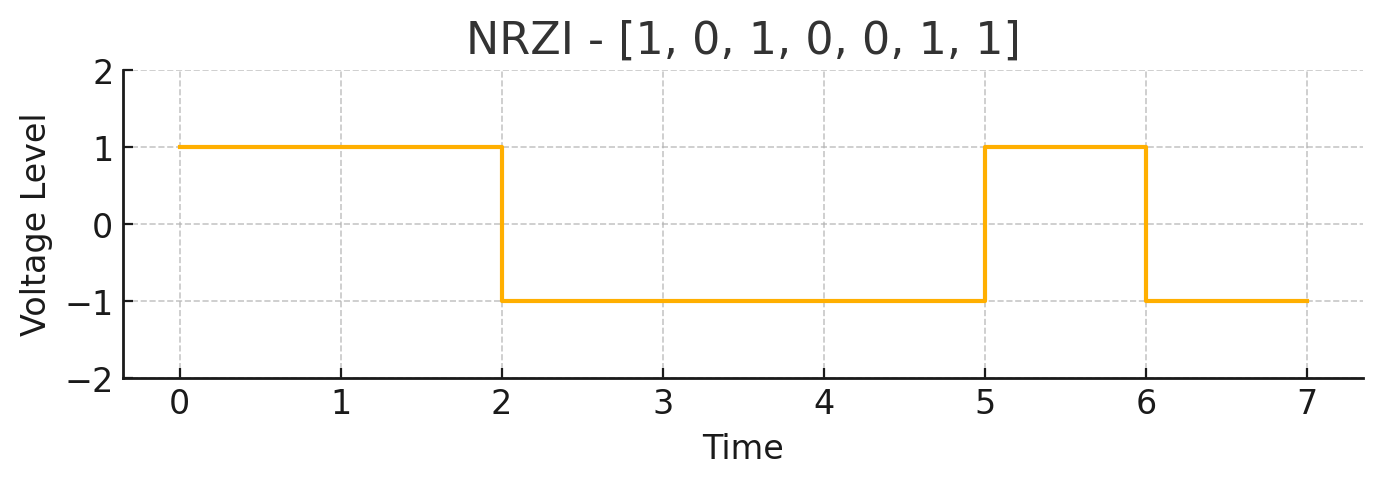
\includegraphics[width=0.85\textwidth]{img/ejercicio_9.png}
\caption{Ejercicio 9: Señal codificada}
\end{figure}
\clearpage


\section*{Ejercicio 10}
Observa una señal codificada con transiciones en el centro de cada bit. ¿Qué codificación podría ser?



\textbf{SOL:} La codificación podría ser Manchester o Manchester Diferencial, ya que ambas presentan transiciones en el centro del intervalo de bit.



\section*{Ejercicio 11}
¿Qué codificación resulta más robusta ante errores de sincronización: NRZ o Manchester Diferencial?



\textbf{SOL:} Manchester Diferencial, porque siempre tiene transiciones, lo que facilita la sincronización incluso si se invierte la polaridad.

\begin{figure}[h!]
\centering
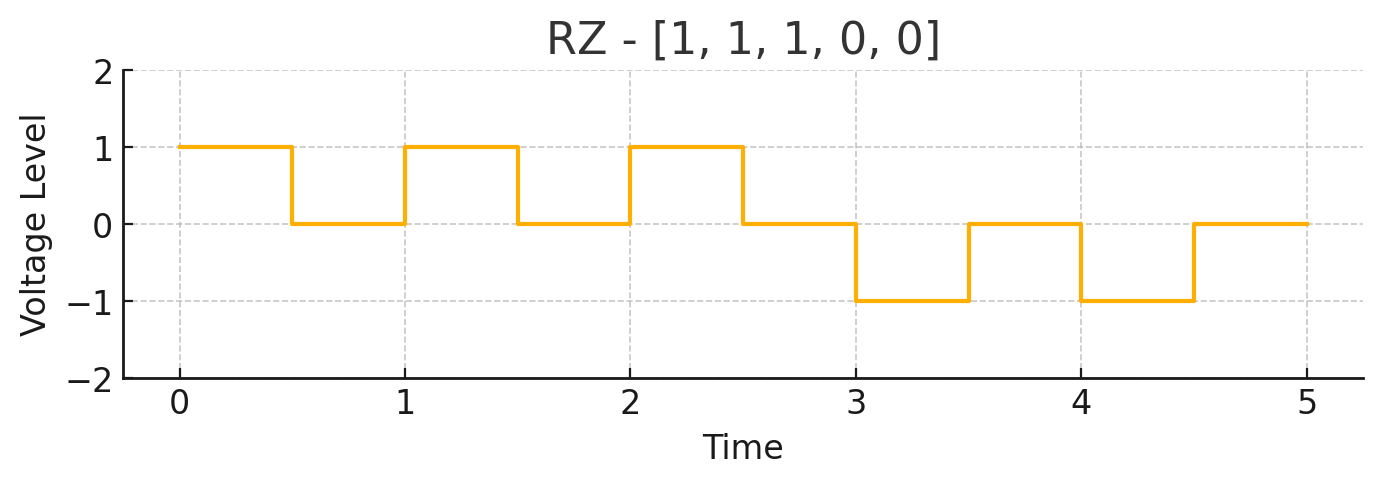
\includegraphics[width=0.85\textwidth]{img/ejercicio_11.png}
\caption{Ejercicio 11: Señal codificada}
\end{figure}
\clearpage




\section*{Ejercicio 13}
En una señal codificada no hay secuencias de más de tres ceros consecutivos. ¿Qué tipo de codificación podría ser?



\textbf{SOL:} Podría tratarse de una codificación 4B/5B, que evita secuencias largas de ceros para mejorar la sincronización.

\begin{figure}[h!]
\centering
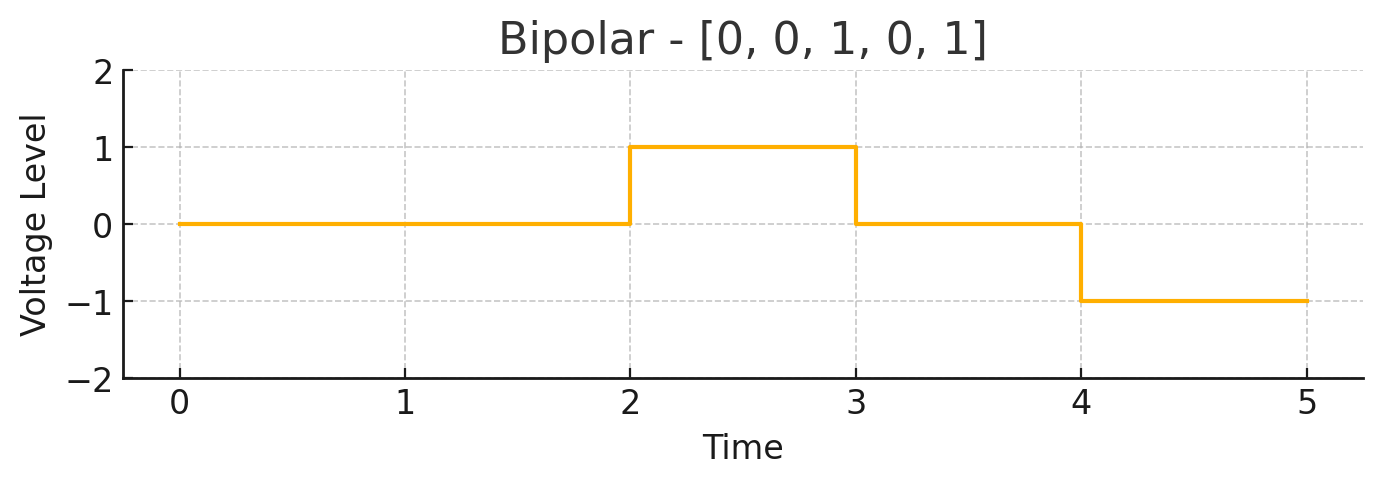
\includegraphics[width=0.85\textwidth]{img/ejercicio_13.png}
\caption{Ejercicio 13: Señal codificada}
\end{figure}
\clearpage



\section*{Ejercicio 15}
Una señal codificada muestra una alternancia constante entre 1 y -1 en los bits '1', mientras los '0' se ven planos. ¿Qué codificación es?



\textbf{SOL:} Es Bipolar (AMI), donde los bits '1' alternan signo y los '0' no generan señal.



\section*{Ejercicio 16}
¿Qué ventaja tiene el uso de codificación RZ frente a NRZ?



\textbf{SOL:} RZ mejora la sincronización al incluir siempre un retorno a cero, aunque usa más ancho de banda.

\end{document}